% Internal diagnostic figures and tables.

\begin{figure}[H]
  \centering
  \includegraphics[width=0.92\linewidth]{appendices/figs/internal/ss3-ts.png}
  \caption{SS3 scenario time series relative to MSY reference points (from curveSS).}
  \label{fig:internal-ss3-ts}
\end{figure}

\begin{figure}[H]
  \centering
  \includegraphics[width=0.92\linewidth]{appendices/figs/internal/ss3-pe-phase.png}
  \caption{Empirical production and curveSS yield curve versus spawning stock biomass.}
  \label{fig:internal-ss3-pe-phase}
\end{figure}

\begin{figure}[H]
  \centering
  \includegraphics[width=0.92\linewidth]{appendices/figs/internal/cpue-fit.png}
  \caption{Observed and expected CPUE indices (sstruth::diagSS).}
  \label{fig:internal-cpue-fit}
\end{figure}

\begin{figure}[H]
  \centering
  \includegraphics[width=0.92\linewidth]{appendices/figs/internal/cpue-residuals.png}
  \caption{CPUE residuals by fleet (sstruth::plotResiduals).}
  \label{fig:internal-cpue-residuals}
\end{figure}

\begin{figure}[H]
  \centering
  \includegraphics[width=0.92\linewidth]{appendices/figs/internal/cpue-std-residuals.png}
  \caption{Standardised CPUE residuals (sstruth::plotStdResiduals).}
  \label{fig:internal-cpue-std-residuals}
\end{figure}

\begin{figure}[H]
  \centering
  \includegraphics[width=0.95\linewidth]{appendices/figs/internal/cpue-runs-test.png}
  \caption{CPUE residual runs tests by fleet (individual-chart criteria; cf. figures.Rmd jara-runs).}
  \label{fig:internal-cpue-runs}
\end{figure}

\begin{figure}[H]
  \centering
  \includegraphics[width=0.95\linewidth]{appendices/figs/internal/cpue-runs-sig3.png}
  \caption{CPUE residual runs tests with 3-sigma limits (ss3diags::SSrunstest).}
  \label{fig:internal-cpue-runs-sig3}
\end{figure}

\begin{figure}[H]
  \centering
  \includegraphics[width=0.88\linewidth]{appendices/figs/internal/ll-components.png}
  \caption{Likelihood components for the reference scenario.}
  \label{fig:internal-ll-components}
\end{figure}

\begin{figure}[H]
  \centering
  \includegraphics[width=0.92\linewidth]{appendices/figs/internal/rec-devs.png}
  \caption{Recruitment deviations for the reference scenario.}
  \label{fig:internal-rec-devs}
\end{figure}

\begin{figure}[H]
  \centering
  \includegraphics[width=0.92\linewidth]{appendices/figs/internal/len-comp-residual-f1.png}
  \caption{Length-composition residuals, fleet 1 (sstruth::ssLen when available).}
  \label{fig:internal-len-comp-residual}
\end{figure}

\begin{figure}[H]
  \centering
  \includegraphics[width=0.88\linewidth]{appendices/figs/internal/ll-profile-total.png}
  \caption{Total log-likelihood profile over M and SR\_surv\_Beta fixed parameters.}
  \label{fig:internal-ll-profile-total}
\end{figure}

\begin{figure}[H]
  \centering
  \includegraphics[width=0.95\linewidth]{appendices/figs/internal/ll-profile-components.png}
  \caption{Likelihood-profile components by data source (M $\times$ SR\_surv\_Beta grid).}
  \label{fig:internal-ll-profile-components}
\end{figure}

\begin{figure}[H]
  \centering
  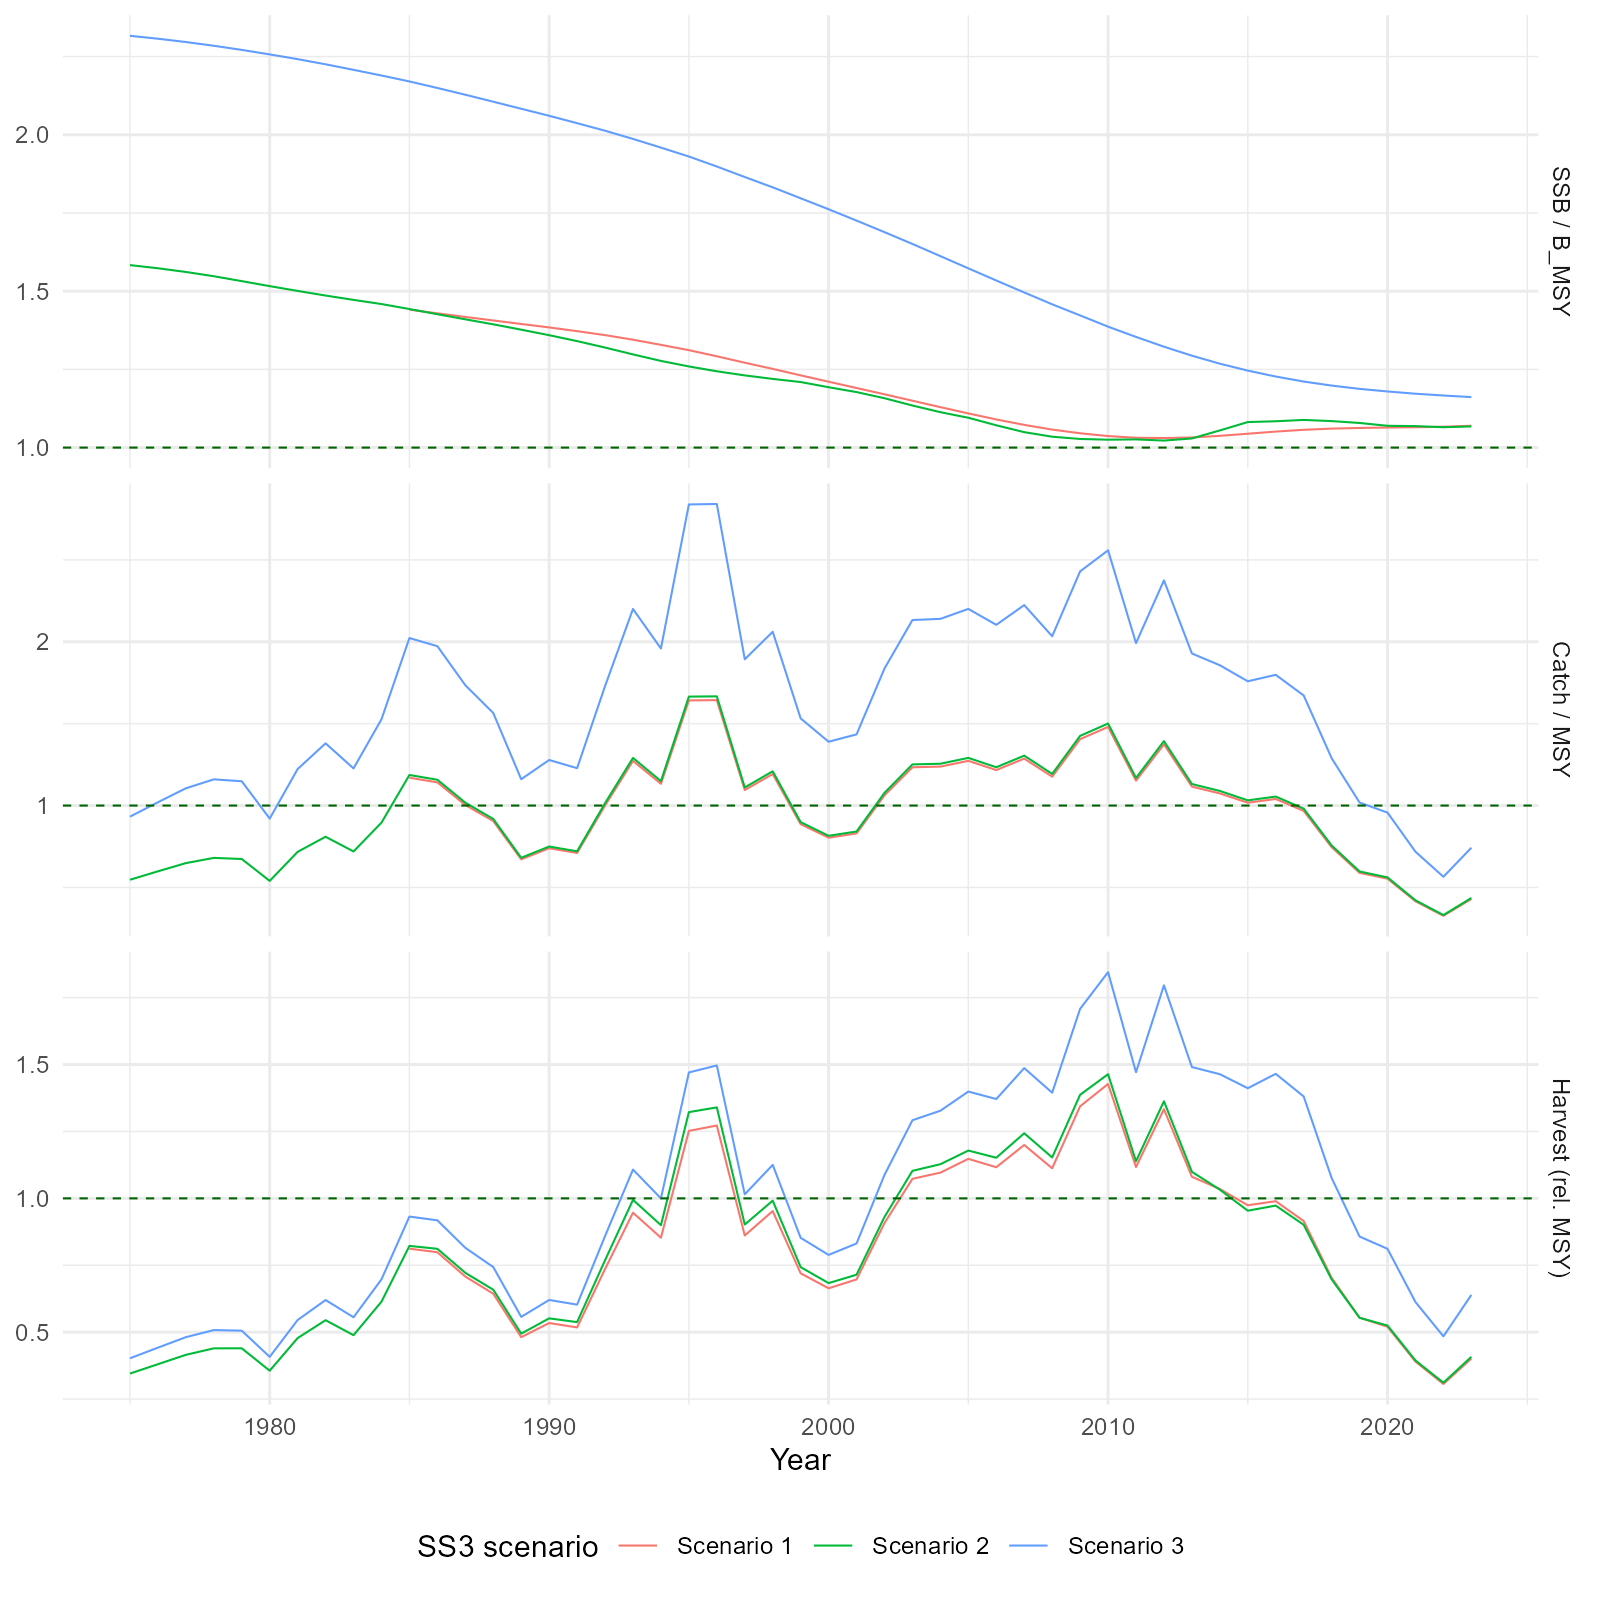
\includegraphics[width=0.92\linewidth]{figs/sma-fig-ts-1.png}
  \caption{sma fig ts 1}
  \label{fig:internal-sma-fig-ts-1}
\end{figure}

\begin{figure}[H]
  \centering
  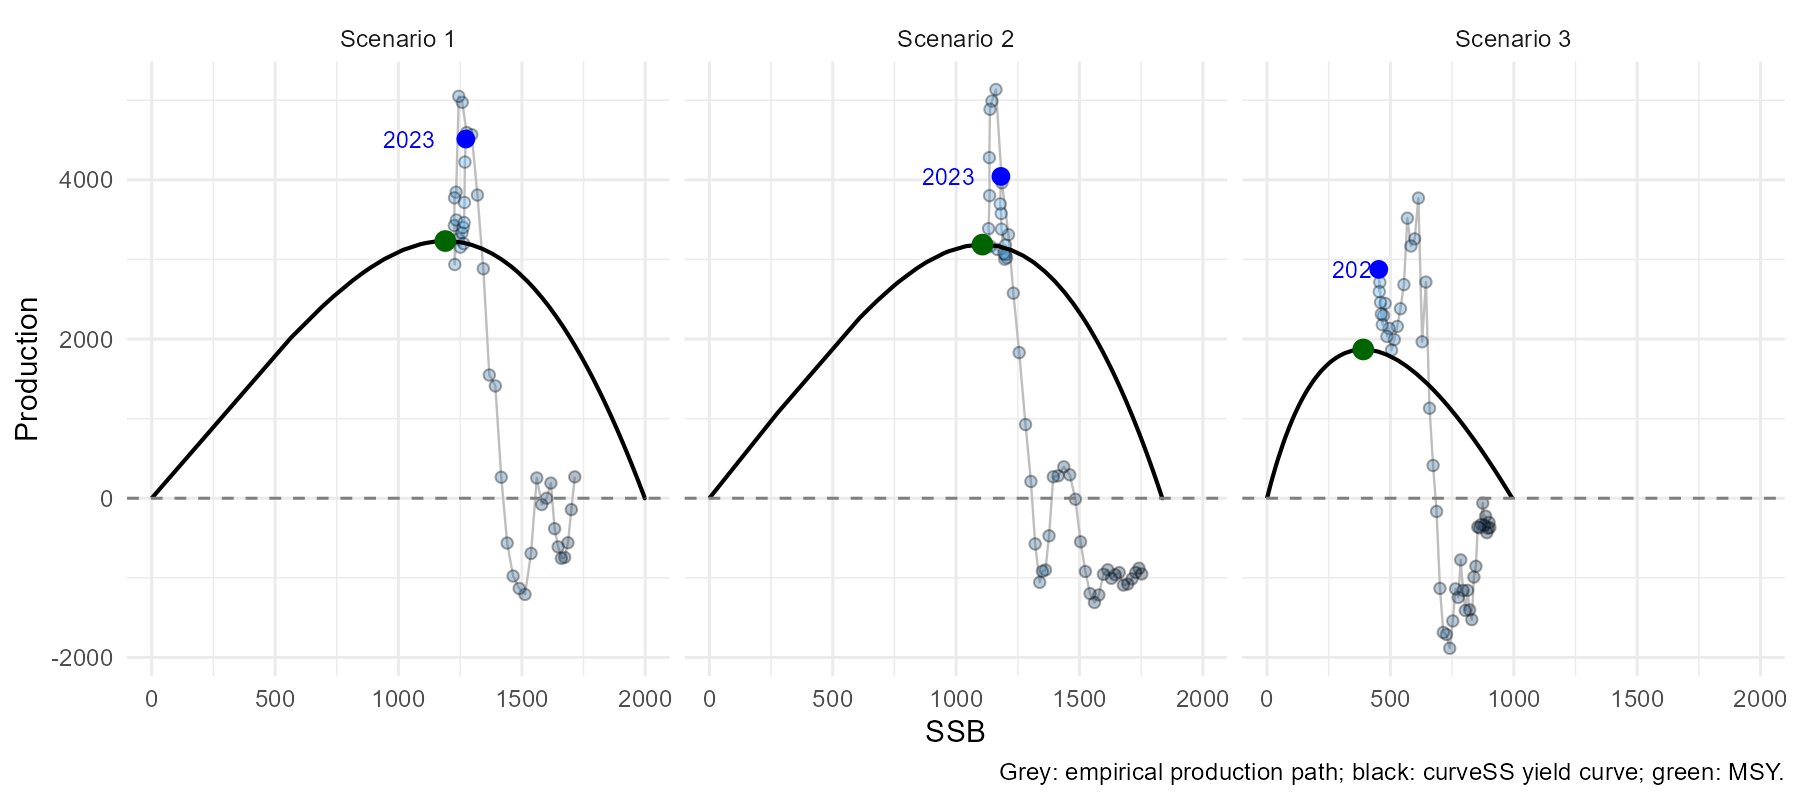
\includegraphics[width=0.92\linewidth]{figs/sma-fig-pe-phase-1.png}
  \caption{sma fig pe phase 1}
  \label{fig:internal-sma-fig-pe-phase-1}
\end{figure}

\begin{figure}[H]
  \centering
  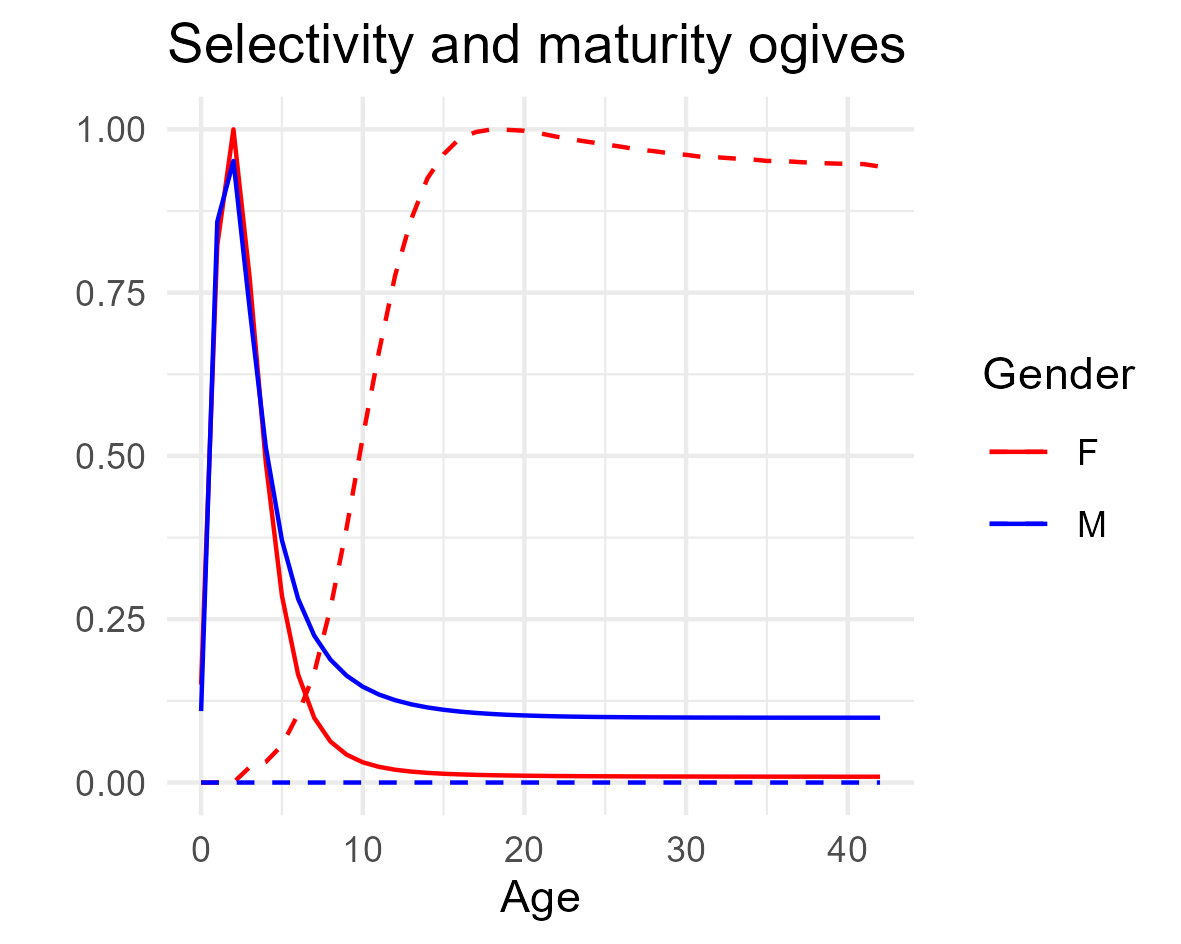
\includegraphics[width=0.92\linewidth]{figs/selmat.png}
  \caption{selmat}
  \label{fig:internal-selmat}
\end{figure}

\begin{figure}[H]
  \centering
  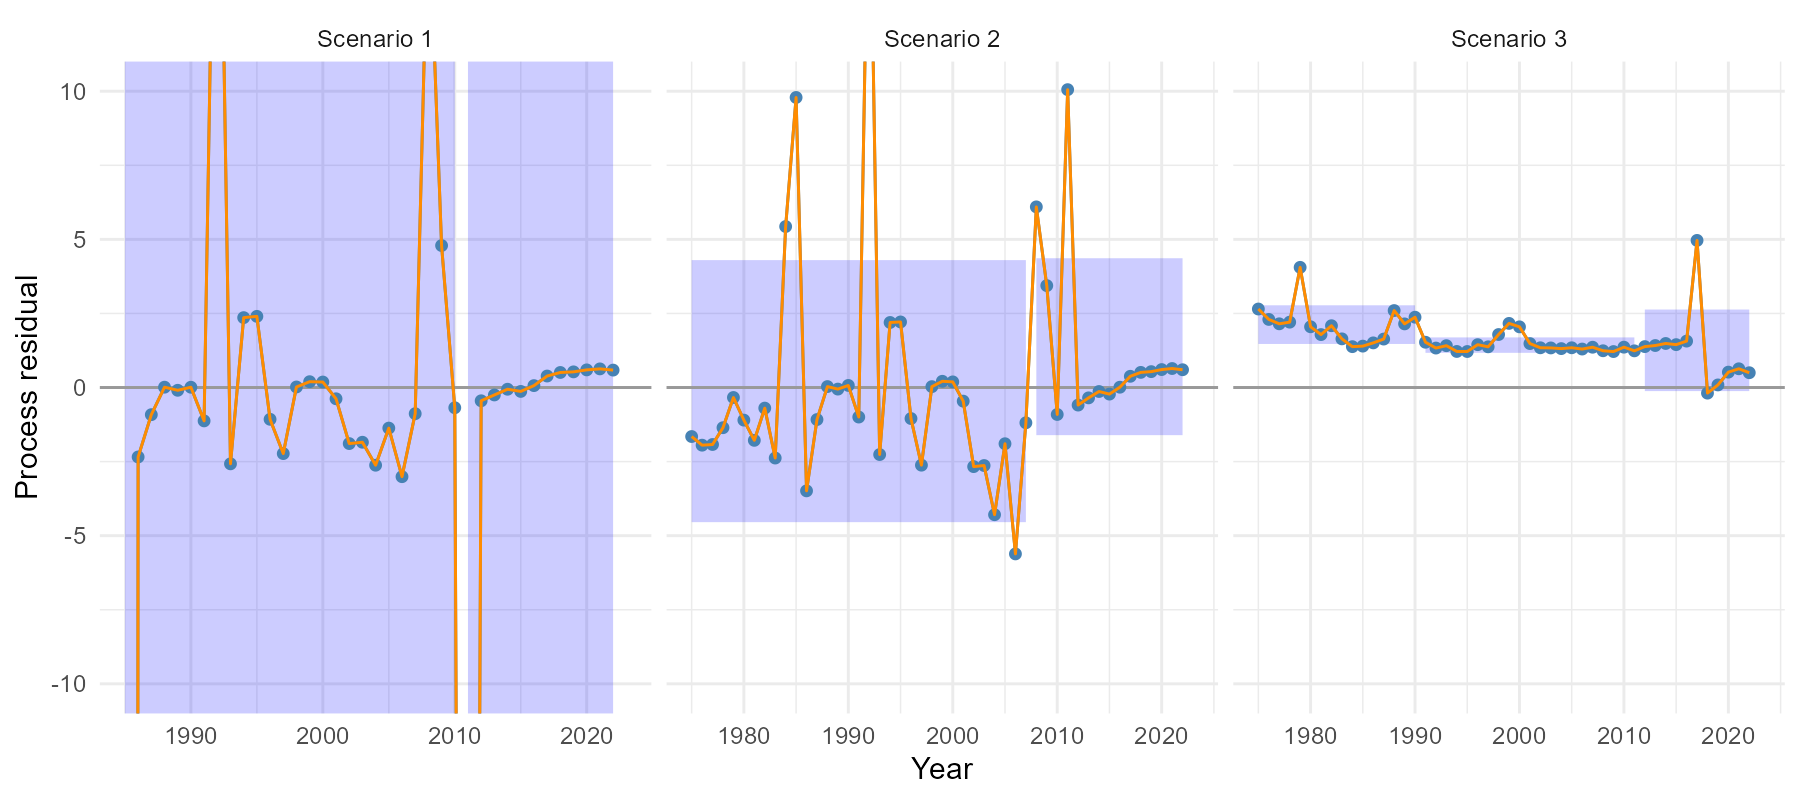
\includegraphics[width=0.92\linewidth]{figs/sma-fig-res-time-1.png}
  \caption{sma fig res time 1}
  \label{fig:internal-sma-fig-res-time-1}
\end{figure}

\begin{figure}[H]
  \centering
  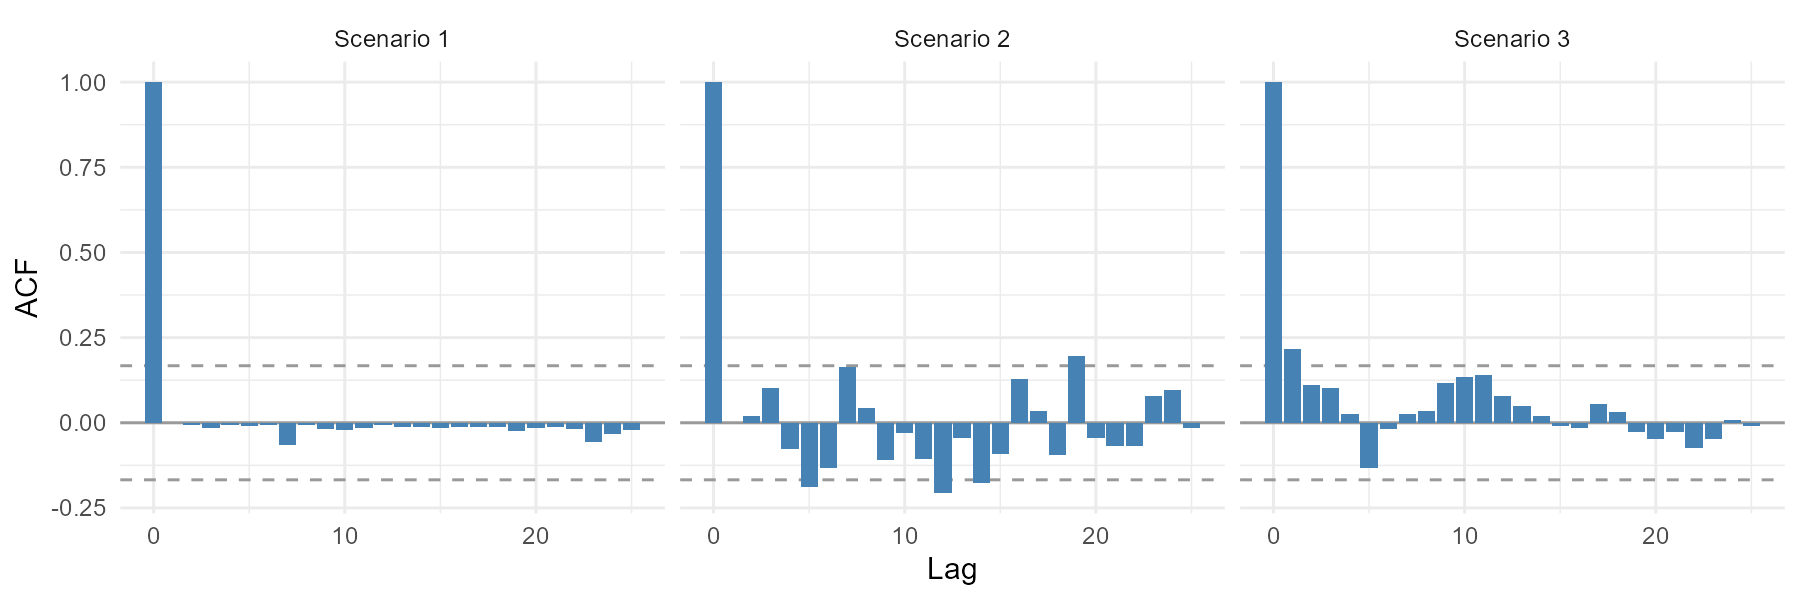
\includegraphics[width=0.92\linewidth]{figs/sma-fig-res-acf-1.png}
  \caption{sma fig res acf 1}
  \label{fig:internal-sma-fig-res-acf-1}
\end{figure}

\begin{figure}[H]
  \centering
  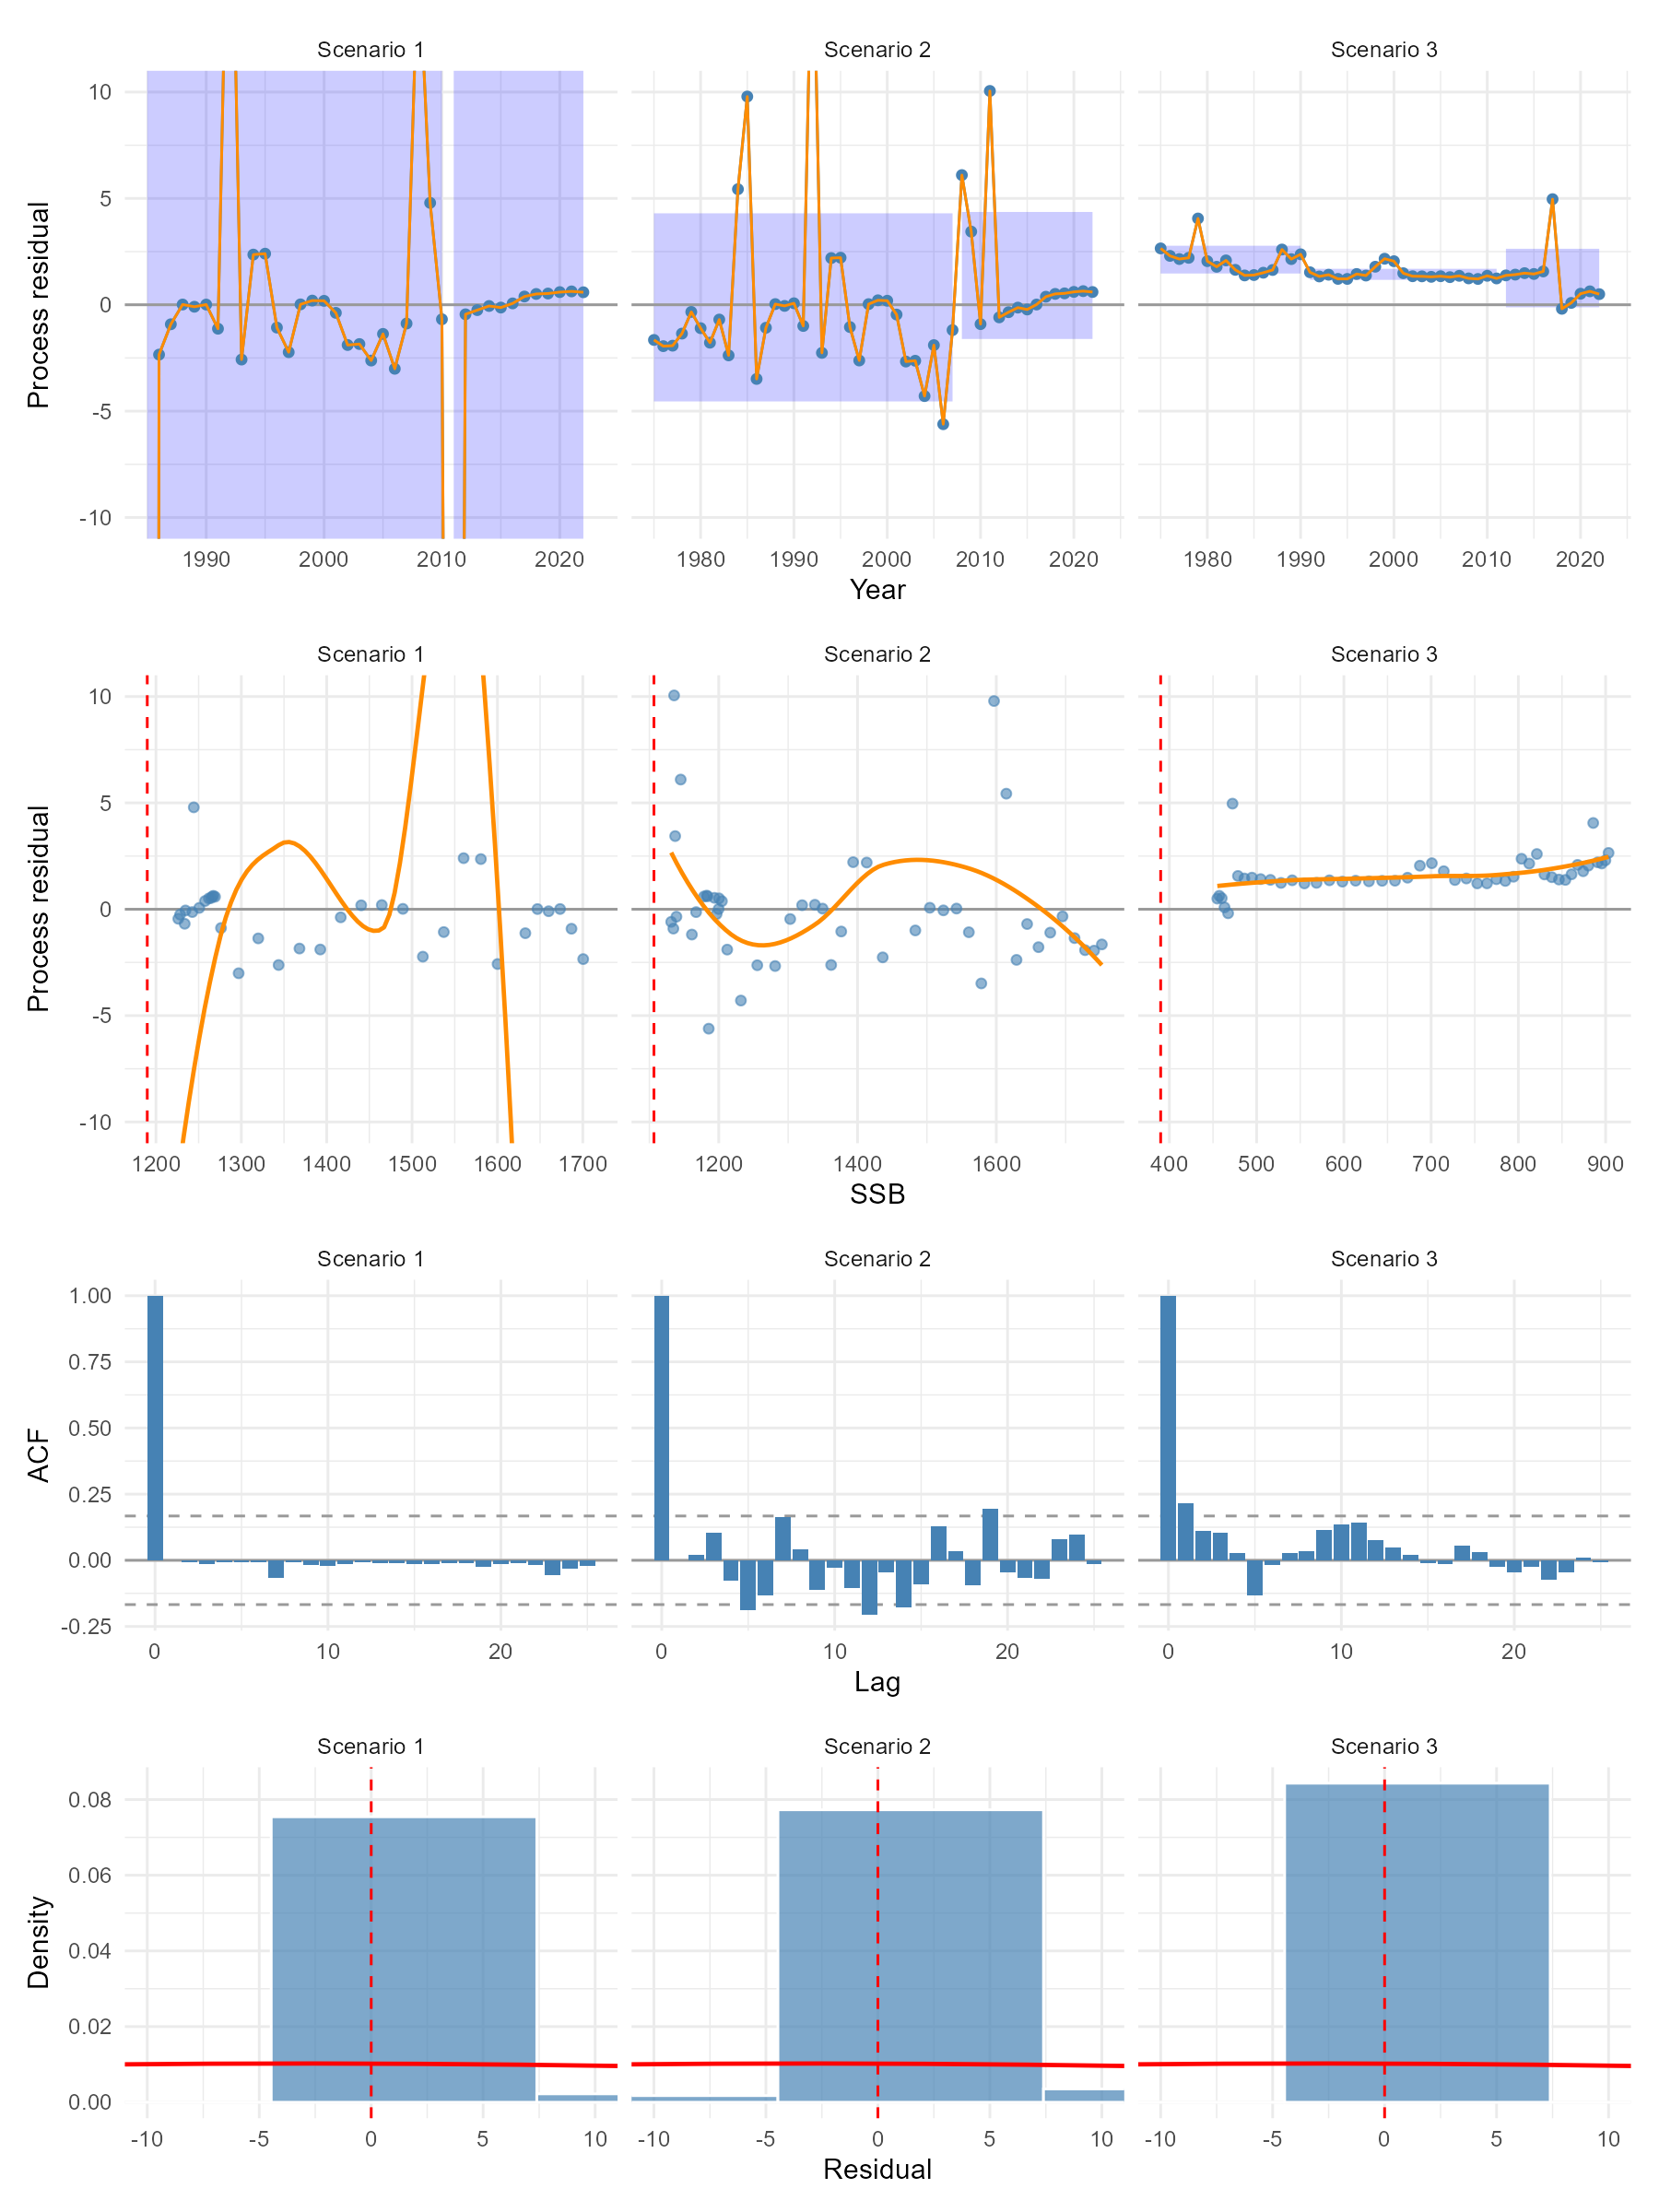
\includegraphics[width=0.92\linewidth]{figs/4panel.png}
  \caption{4panel}
  \label{fig:internal-4panel}
\end{figure}

